% Slug: visual-unroll-tail
% Source: figures/unroll-tail.tex:3 (tikzpicture env start line)
% Original label: \label{fig:visual-unroll-tail}
% Original caption (LaTeX source):
%   Two full groups and a two-iteration tail cover ten iterations once each, preserving their original order.
% Original caption (plain text):
%   Two full groups and a two-iteration tail cover ten iterations once each, preserving their original order.
% Required TikZ setup: \usepackage{tikz} + \usetikzlibrary{arrows.meta, positioning, shapes.geometric, fit} (loaded by support/compiler-pseudocode.sty).
% Shared styles used in this picture: (none of the shared styles; plain TikZ only).
%   Defined in support/compiler-pseudocode.sty: `basic block', `cfg edge', `back edge', `block label'.
% Usage: % Slug: visual-unroll-tail
% Source: figures/unroll-tail.tex:3 (tikzpicture env start line)
% Original label: \label{fig:visual-unroll-tail}
% Original caption (LaTeX source):
%   Two full groups and a two-iteration tail cover ten iterations once each, preserving their original order.
% Original caption (plain text):
%   Two full groups and a two-iteration tail cover ten iterations once each, preserving their original order.
% Required TikZ setup: \usepackage{tikz} + \usetikzlibrary{arrows.meta, positioning, shapes.geometric, fit} (loaded by support/compiler-pseudocode.sty).
% Shared styles used in this picture: (none of the shared styles; plain TikZ only).
%   Defined in support/compiler-pseudocode.sty: `basic block', `cfg edge', `back edge', `block label'.
% Usage: % Slug: visual-unroll-tail
% Source: figures/unroll-tail.tex:3 (tikzpicture env start line)
% Original label: \label{fig:visual-unroll-tail}
% Original caption (LaTeX source):
%   Two full groups and a two-iteration tail cover ten iterations once each, preserving their original order.
% Original caption (plain text):
%   Two full groups and a two-iteration tail cover ten iterations once each, preserving their original order.
% Required TikZ setup: \usepackage{tikz} + \usetikzlibrary{arrows.meta, positioning, shapes.geometric, fit} (loaded by support/compiler-pseudocode.sty).
% Shared styles used in this picture: (none of the shared styles; plain TikZ only).
%   Defined in support/compiler-pseudocode.sty: `basic block', `cfg edge', `back edge', `block label'.
% Usage: % Slug: visual-unroll-tail
% Source: figures/unroll-tail.tex:3 (tikzpicture env start line)
% Original label: \label{fig:visual-unroll-tail}
% Original caption (LaTeX source):
%   Two full groups and a two-iteration tail cover ten iterations once each, preserving their original order.
% Original caption (plain text):
%   Two full groups and a two-iteration tail cover ten iterations once each, preserving their original order.
% Required TikZ setup: \usepackage{tikz} + \usetikzlibrary{arrows.meta, positioning, shapes.geometric, fit} (loaded by support/compiler-pseudocode.sty).
% Shared styles used in this picture: (none of the shared styles; plain TikZ only).
%   Defined in support/compiler-pseudocode.sty: `basic block', `cfg edge', `back edge', `block label'.
% Usage: \input{graphs-code/visual-unroll-tail.tikz.tex} inside a figure environment
%   (wrap with \begin{figure} ... \caption{...} \label{fig:visual-unroll-tail} ... \end{figure}).
% Note: tikzpicture body below is verbatim from the source; do not reformat.
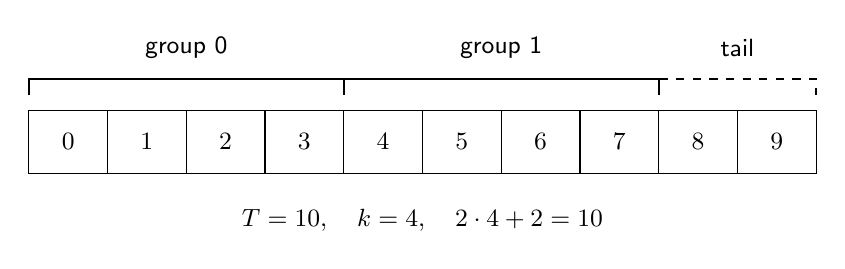
\begin{tikzpicture}[x=10mm,y=10mm]
    \foreach \i in {0,...,9} {
      \draw (\i,0) rectangle +(1,0.8);
      \node[font=\small] at (\i+0.5,0.4) {\i};
    }
    \draw[thick] (0,1) -- (0,1.2) -- (4,1.2) -- (4,1);
    \draw[thick] (4,1) -- (4,1.2) -- (8,1.2) -- (8,1);
    \draw[dashed,thick] (8,1) -- (8,1.2) -- (10,1.2) -- (10,1);
    \node[font=\sffamily\small] at (2,1.6) {group 0};
    \node[font=\sffamily\small] at (6,1.6) {group 1};
    \node[font=\sffamily\small] at (9,1.6) {tail};
    \node[font=\small] at (5,-0.6) {$T=10,\quad k=4,\quad 2\cdot4+2=10$};
  \end{tikzpicture}
 inside a figure environment
%   (wrap with \begin{figure} ... \caption{...} \label{fig:visual-unroll-tail} ... \end{figure}).
% Note: tikzpicture body below is verbatim from the source; do not reformat.
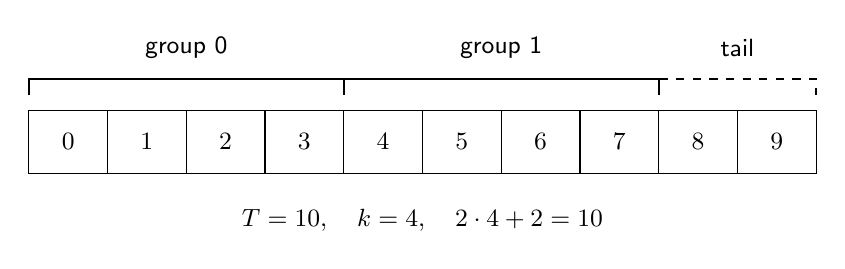
\begin{tikzpicture}[x=10mm,y=10mm]
    \foreach \i in {0,...,9} {
      \draw (\i,0) rectangle +(1,0.8);
      \node[font=\small] at (\i+0.5,0.4) {\i};
    }
    \draw[thick] (0,1) -- (0,1.2) -- (4,1.2) -- (4,1);
    \draw[thick] (4,1) -- (4,1.2) -- (8,1.2) -- (8,1);
    \draw[dashed,thick] (8,1) -- (8,1.2) -- (10,1.2) -- (10,1);
    \node[font=\sffamily\small] at (2,1.6) {group 0};
    \node[font=\sffamily\small] at (6,1.6) {group 1};
    \node[font=\sffamily\small] at (9,1.6) {tail};
    \node[font=\small] at (5,-0.6) {$T=10,\quad k=4,\quad 2\cdot4+2=10$};
  \end{tikzpicture}
 inside a figure environment
%   (wrap with \begin{figure} ... \caption{...} \label{fig:visual-unroll-tail} ... \end{figure}).
% Note: tikzpicture body below is verbatim from the source; do not reformat.
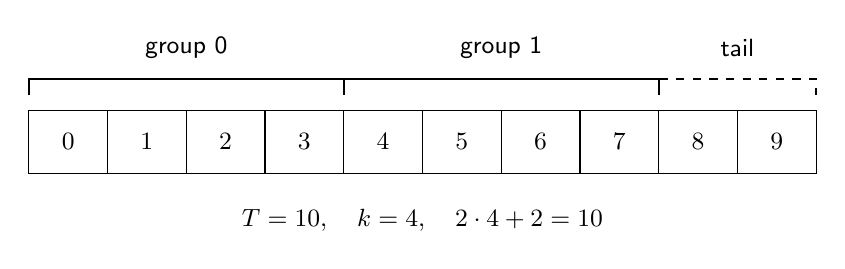
\begin{tikzpicture}[x=10mm,y=10mm]
    \foreach \i in {0,...,9} {
      \draw (\i,0) rectangle +(1,0.8);
      \node[font=\small] at (\i+0.5,0.4) {\i};
    }
    \draw[thick] (0,1) -- (0,1.2) -- (4,1.2) -- (4,1);
    \draw[thick] (4,1) -- (4,1.2) -- (8,1.2) -- (8,1);
    \draw[dashed,thick] (8,1) -- (8,1.2) -- (10,1.2) -- (10,1);
    \node[font=\sffamily\small] at (2,1.6) {group 0};
    \node[font=\sffamily\small] at (6,1.6) {group 1};
    \node[font=\sffamily\small] at (9,1.6) {tail};
    \node[font=\small] at (5,-0.6) {$T=10,\quad k=4,\quad 2\cdot4+2=10$};
  \end{tikzpicture}
 inside a figure environment
%   (wrap with \begin{figure} ... \caption{...} \label{fig:visual-unroll-tail} ... \end{figure}).
% Note: tikzpicture body below is verbatim from the source; do not reformat.
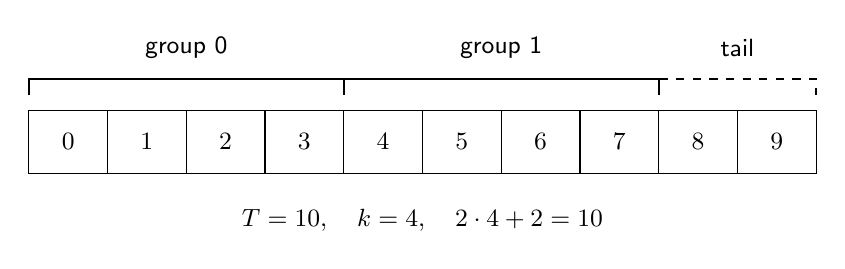
\begin{tikzpicture}[x=10mm,y=10mm]
    \foreach \i in {0,...,9} {
      \draw (\i,0) rectangle +(1,0.8);
      \node[font=\small] at (\i+0.5,0.4) {\i};
    }
    \draw[thick] (0,1) -- (0,1.2) -- (4,1.2) -- (4,1);
    \draw[thick] (4,1) -- (4,1.2) -- (8,1.2) -- (8,1);
    \draw[dashed,thick] (8,1) -- (8,1.2) -- (10,1.2) -- (10,1);
    \node[font=\sffamily\small] at (2,1.6) {group 0};
    \node[font=\sffamily\small] at (6,1.6) {group 1};
    \node[font=\sffamily\small] at (9,1.6) {tail};
    \node[font=\small] at (5,-0.6) {$T=10,\quad k=4,\quad 2\cdot4+2=10$};
  \end{tikzpicture}
